\section{Problem Setup}

\subsection{Task Formulation}

The dataset $\mathcal{D}$ consists of premises $\mathcal{P}$, conditions $\mathcal{C}=\{entailment, neutral, contradiction\}$ and hypotheses $\mathcal{H}$. Each sample $s_i$ is a tuple $(p^i, c^i, h^i)$, where $p^i \in \mathcal{P}$, $c^i \in \mathcal{C}$ and $h^i \in \mathcal{H}$. The NLI generation task is defined as: Given premise $p$ and condition $c$, predict hypothesis $h$. This formulation is the same as ~\citet{DBLP:journals/csl/StarcM17} except we assume there are only $K$
samples for per condition in training set $\mathcal{D}_{train}$ and development set $\mathcal{D}_{dev}$. This is following the few-shot settings in ~\citet{DBLP:conf/acl/GaoFC20}.

\subsection{Evaluation protocol}

Previous works show the performance of models fine-tuned on the small dataset is largely affected by the data split and hyper-parameters~\citep{DBLP:journals/corr/abs-2002-06305,DBLP:conf/iclr/0007WKWA21}. 
To address this issue, we use the same evaluation protocol in 
\citet{DBLP:conf/acl/GaoFC20}. We measure the average performance on 
5 different randomly sampled $\mathcal{D}_{train}$ and $\mathcal{D}_{dev}$ 
splits. The hyper-parameters are chosen by the performance in 
$\mathcal{D}_{dev}$ for each split.

\begin{figure*}
	\centering
	\scalebox{1.0}{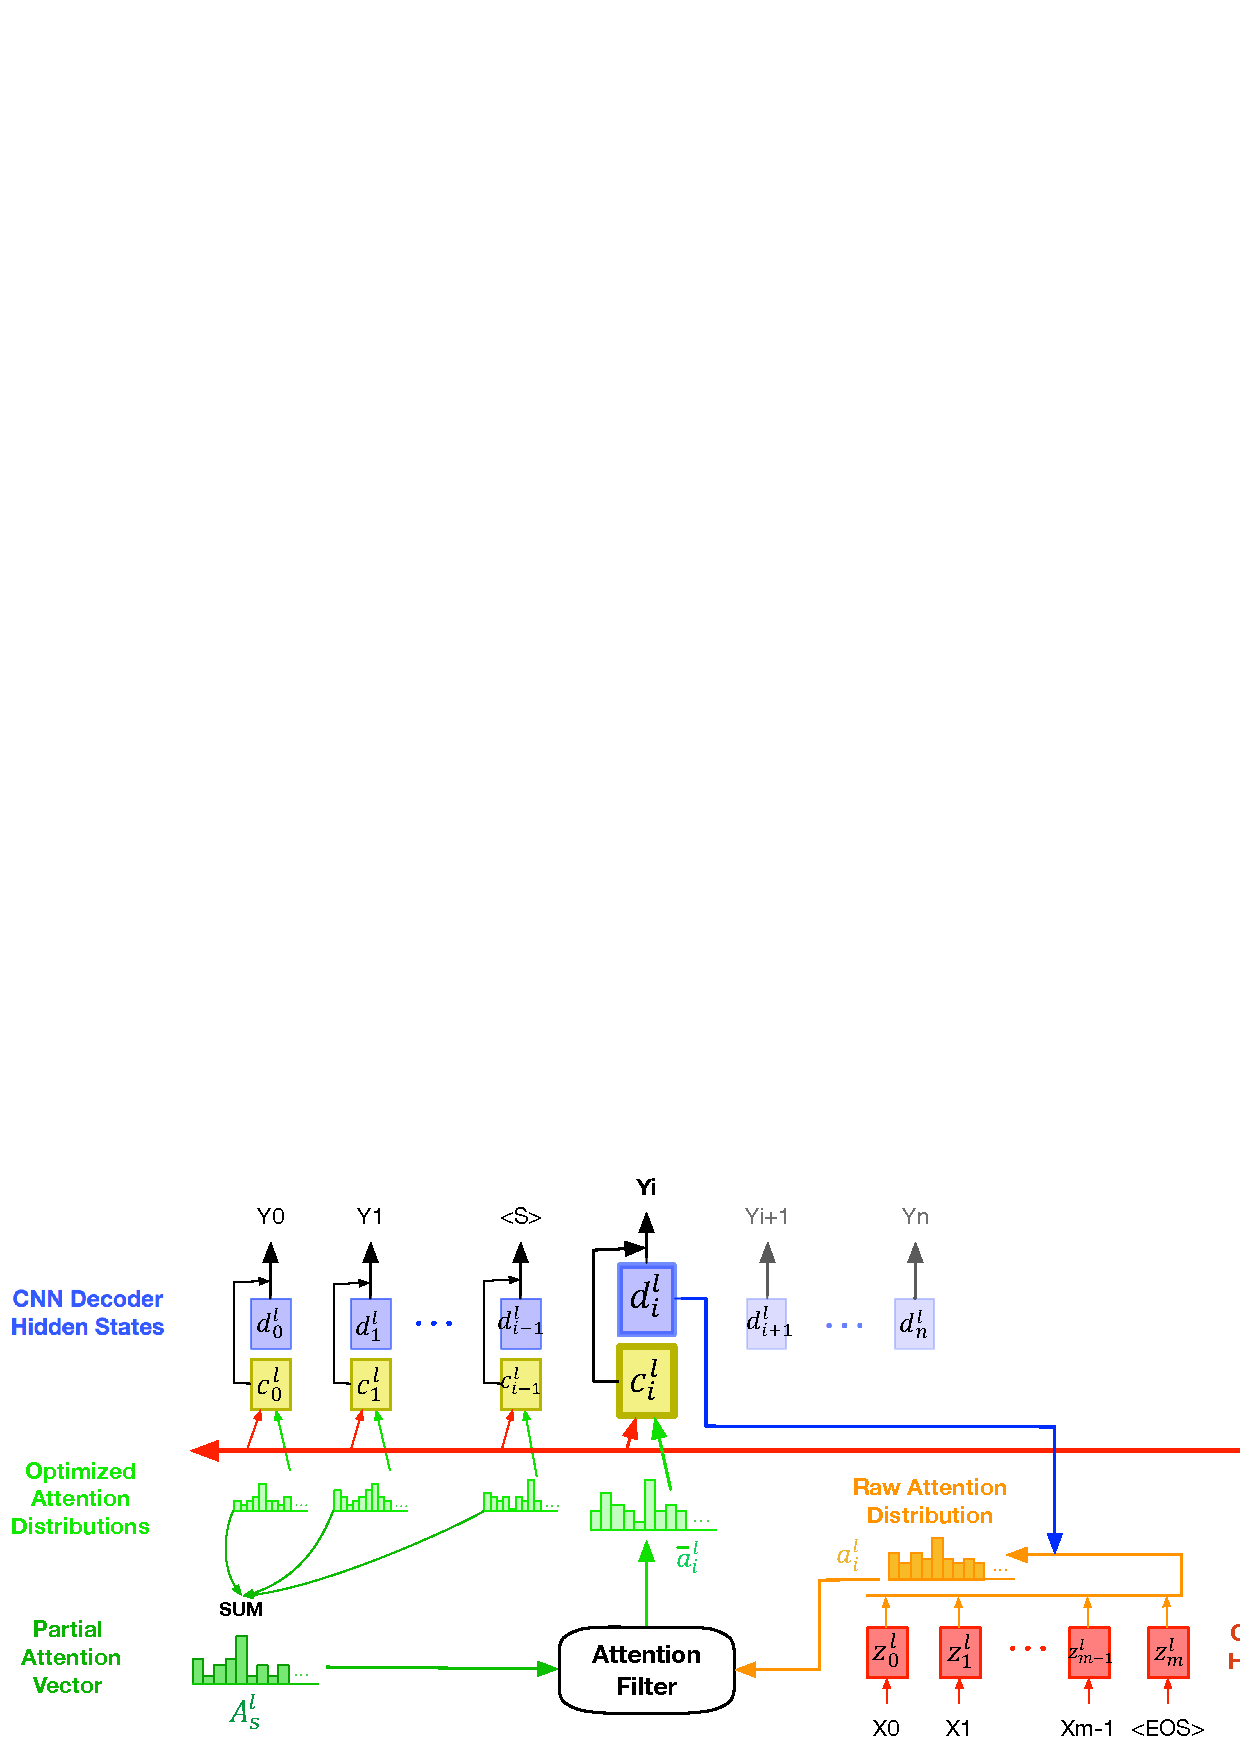
\includegraphics[width=1.7\columnwidth]{figure/model.pdf}}
	\caption{An illustration of our LM-PDD. The blue dash line is the first stage: prompt template auto-generation, while the dark line stands for the dynamic demonstration training in stage two.}
	\label{fig:model}
\end{figure*}
